% D.6 K 字形：等腰直角△ABC（∠C=90°，AC=BC），过 C 直线 l，A、B 作 l 的垂线 → M、N
\documentclass[tikz,border=4pt]{standalone}
\usepackage{ctex}
\usepackage{amsmath}
\usetikzlibrary{calc}
\begin{document}
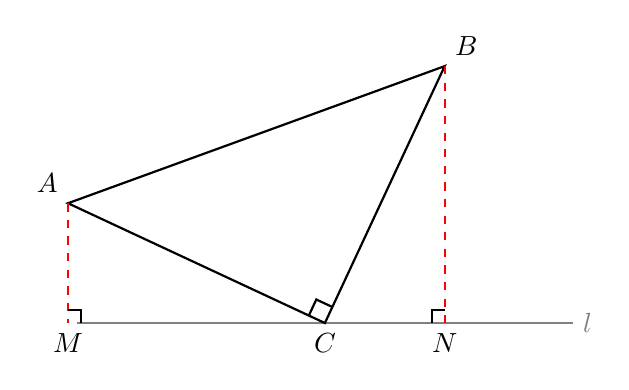
\begin{tikzpicture}[scale=0.9, thick]
  \coordinate (C) at (0, 0);
  % 直线 l 沿 x 轴方向
  \coordinate (Lstart) at (-3.5, 0);
  \coordinate (Lend)   at ( 3.5, 0);

  % AC=BC，∠ACB=90°；让 CA 与 l 成 25°，CB 与 l 成 115°
  \coordinate (A) at ({4*cos(155)}, {4*sin(155)});
  \coordinate (B) at ({4*cos(65)},  {4*sin(65)});
  % M = A 在 l 上的投影；N = B 在 l 上的投影
  \coordinate (M) at ({4*cos(155)}, 0);
  \coordinate (N) at ({4*cos(65)},  0);

  \draw[gray] (Lstart) -- (Lend) node[right] {$l$};
  \draw (A) -- (C) -- (B) -- cycle;
  \draw[red, dashed] (A) -- (M);
  \draw[red, dashed] (B) -- (N);

  % 直角符号 at C
  \draw ($(C) + ({0.25*cos(155)}, {0.25*sin(155)})$)
     -- ($(C) + ({0.25*cos(155)+0.25*cos(65)}, {0.25*sin(155)+0.25*sin(65)})$)
     -- ($(C) + ({0.25*cos(65)},  {0.25*sin(65)})$);
  % 直角符号 at M
  \draw ($(M)+(0.18,0)$) -- ($(M)+(0.18,0.18)$) -- ($(M)+(0,0.18)$);
  % 直角符号 at N
  \draw ($(N)+(-0.18,0)$) -- ($(N)+(-0.18,0.18)$) -- ($(N)+(0,0.18)$);

  \node[above left]  at (A) {$A$};
  \node[above right] at (B) {$B$};
  \node[below]       at (C) {$C$};
  \node[below]       at (M) {$M$};
  \node[below]       at (N) {$N$};
\end{tikzpicture}
\end{document}
